\chapter{Architetture}

Dopo aver definito i requisiti dell'applicazione è stato realizzato un prototipo funzionante utilizzando un'architettura three tier come da figura \ref{fig:app-version-1}.
Durante lo sviluppo del lavoro sono state sperimentate alcune architetture con il fine di mostrare una possibile evoluzione di un'applicazione da una versione monolitica ad una a microservizi.

\begin{figure}[h]
	\centering
	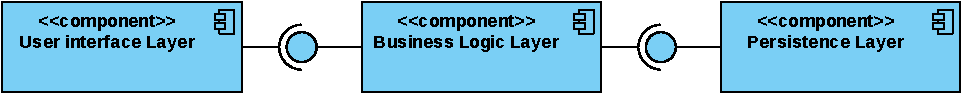
\includegraphics[width=\textwidth]{img/architecture-01}
	\caption{Architettura della prima versione dell'applicazione}
	\label{fig:app-version-1}
\end{figure}

Scelta un'architettura
In particolare  in questo capitolo saranno descritte , e sarà presentata la versione selezionata per la realizzazione dell'applicazione in esame.

Il cuore di un software object-oriented si trova nel modello di dominio. Questo raccoglie i concetti estratti dall'analisi dei requisiti ed è composto da una rete di oggetti dotati di attributi e metodi che rispecchiano i dati da memorizzare e le operazioni necessarie alla loro elaborazione.
Non vi è di base alcun legame con tecnologie particolari, cosa che permette di evitare l'inserimento all'interno di questi oggetti di caratteristiche finalizzate per esempio alla memorizzazione su un certo tipo di database, alla visualizzazione su un certo tipo di interfaccia o all'invio su un certo tipo di canale.\\
Scrivere il codice di supporto direttamente all'interno degli oggetti del modello di dominio, o spostare parte della logica all'interno dei componenti UI o nelle procedure relative al database abbassa in maniera critica la manutenibilità del codice: le varie componenti sono legate tra loro, e devono evolvere necessariamente in contemporanea.
Il test automatico diventa complesso, e si rischia di raggiungere presto lo stato di \textit{big ball of mud}\cite{microservices_architecture}.
Scrivere codice il più possibile disaccoppiato dalle tecnologie di contorno lo rende più manutenibile e testabile, ma può diminuire la produttività del team di sviluppo, soprattutto quando l'applicazione da sviluppare non è di eccessiva complessità.
\'E quindi necessario trovare un compromesso, si può essere tentati di 

Sono state studiate numerose architetture che separano il codice a seconda della responsabilità.
Una di queste è l'architettura a livelli.

\section{Layered architecture}

Questo tipo di architettura è uno degli standard più affermati nello sviluppo di applicazioni enterprise.\\
Il codice è organizzato a livelli sovrapposti, ognuno dei quali può sfruttare i servizi esposti \textbf{soltanto} dai quelli sottostanti.
Esistono una serie di layers standard, di seguito se ne riportano alcuni dei più comuni\cite{ddd}:
\begin{itemize}
	\item Presentation: Fornisce informazioni e interpreta i comandi provenienti dall'esterno, in modo da interfacciarsi con un utente o un'altro software.
	\item Application: Sottile strato che dirige la logica di dominio delegando le azioni ai business objects.
	\item Model: Mantiene lo stato della logica di dominio e contiene le regole che la governano. \'E il cuore del software.
	\item Infrastructure: Fornisce funzionalità utili agli altri strati come persistenza, invio di messaggi, creazione interfaccia grafica ecc...
\end{itemize}
In questa visione il livello di business logic è consapevole dei livelli sottostanti, ed interagisce direttamente con essi.
Dovendo gestire più ad alto livello la logica di dominio, per esempio aprendo e chiudendo una transazione, anche il livello application necessita di interagire con lo strato di infrastruttura.

Le linee guida per realizzare un'applicazione seguendo questa architettura prevedono di partizionare il codice in livelli coesi e dipendenti solamente da quelli sottostanti.
Gli oggetti del modello di dominio devono essere indipendenti dalle varie rappresentazioni, che siano destinate ad UI, persistenza o altro, in modo da essere concentrati sul rappresentare efficacemente quello per cui sono stati pensati.\\
La separazione in layers permette inoltre di poter effettuare il rilascio delle varie parti dell'applicazione su macchine differenti, favorendone l'evoluzione e la scalabilità.

Esistono varie versioni di questa architettura, in cui i livelli di contorno variano: una di queste è la 3-layered architecture, che prevede i livelli di \textit{Presentation} per la gestione della UI, \textit{Model} per la logica di dominio e \textit{Persistence} per dialogare con i database.
Questi sono sufficienti per gran parte della applicazioni enterprise.\\
\'E stato possibile distillare questa struttura anche grazie a tecnologie come Hibernate, i moderni application server o i framework per UI: come mostrato in figura \ref{3-tiers-2}//TODO il vero livello di presentazione può essere realizzato indipendentemente dal resto e con un linguaggio diverso; questo comunicherà con il software tramite servizi remoti (es. REST), i quali formeranno il livello di Application e gestiranno in modo dichiarativo le transazioni. Rimangono il livello di business logic e quello di persistenza, spesso legati nel caso si utilizzi una tecnologia come JPA, che decora gli oggetti appartenenti al modello con annotazioni specifiche, poco invasive, parte della specifica Java.


//TODO

Quando si parla di realizzare la logica di dominio per un'applicazione enterprise vi sono numerosi approcci che si possono adottare: di seguito riportiamo due patterns notevoli\cite{enterprise_app}:\\
\textbf{Transaction script:} Si pone la logica di dominio in oggetti esterni al modello: questo permette di avere entità più leggere, facilmente mappabili su un database.

\textbf{Domain model:} La logica di dominio è contenuta quasi interamente all'interno degli oggetti del modello: ciò permette di avere classi più ricche, anche se più difficilmente mappabili su di un database.

Il primo approccio è adatto quando la complessità di ciò che si deve realizzare non è elevata, in quanto la separazione tra livelli diventa più labile, riducendo la manutenibilità del codice.


\section{Ports and adapters}

Una delle alternative all'architettura organizzata a \textit{layers} è l'architettura chiamata \textit{ports and adapters} o \textit{hexagonal architecture}\cite{microservices_architecture}.

\begin{figure}[h]
	\centering
	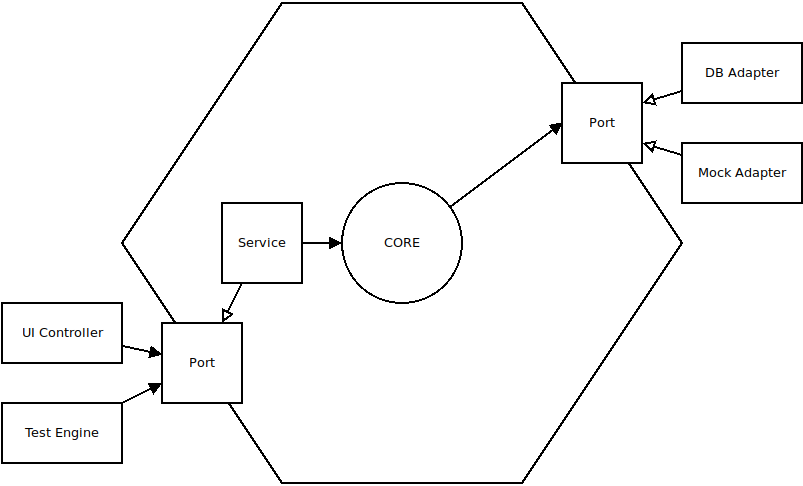
\includegraphics[scale=0.5]{img/hexagonal}
	\caption{Modulo ad architettura ports and adapters}
	\label{fig:hexagonal}
\end{figure}

Anche in questo caso si cerca di rendere il più possibile indipendente il nucleo di un'applicazione dalle tecnologie di contorno, come database, sistema di scambio messaggi ecc...
Le comunicazioni di input/output con l'esterno sono guidate da interfacce \textbf{definite dal nucleo} e chiamate \textit{porte}: queste possono essere di tipo \textit{inbound} quando un modulo esterno ha necessità di invocare la logica di dominio, o di tipo \textit{outbound} quando il nucleo ha la necessità di invocare servizi esterni.

Ogni porta è implementata da uno o più adattatori (\textit{adapters}) a seconda delle esigenze: per esempio una \textit{outbound port} per l'accesso ad un repository di dati può essere concretizzata sia da un adattatore legato ad un DBMS che da uno dedicato al testing.

Convertire un'applicazione service oriented realizzata a layers in una aderente all'architettura esagonale non è un'operazione complessa: se per esempio lo stack è di tipo 3-tier con una serie di servizi REST esposti che invocano internamente la logica di dominio ed uno strato di persistenza (es: JPA), la separazione tra core e adapters è immediata (vedi figura \ref{fig:hexagonal_3_tier}).

\begin{figure}[h]
	\centering
	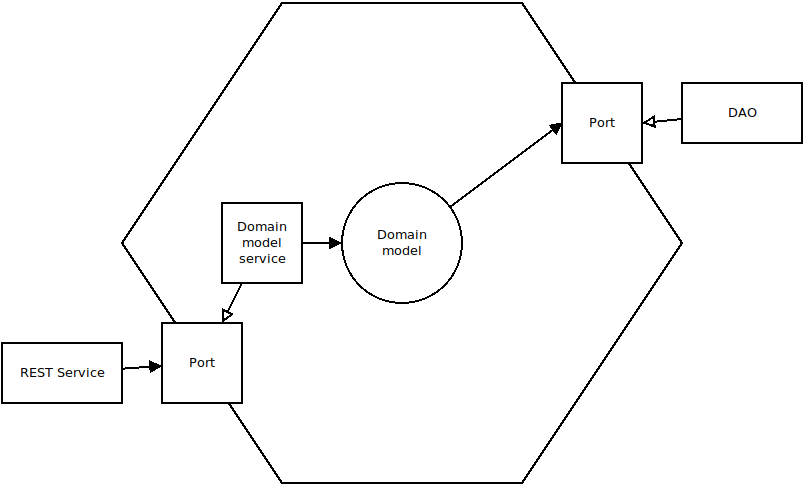
\includegraphics[scale=0.5]{img/hexagonal_3_tier}
	\caption{Conversione 3-tier - ports/adapters}
	\label{fig:hexagonal_3_tier}
\end{figure}

I benefici di tale architettura diventano evidenti quando utilizzata all'interno di un software a microservizi, in quanto è possibile identificare con più chiarezza il compito del modulo e questo è testabile con maggior facilità.

\subsection{Architettura del software}
Il sistema è stato realizzato separando lo strato di UI da quello di business logic, realizzando secondo i principi dell'architettura \textit{ports/adapters}.\\
In particolare sono esposti verso l'esterno (inbound) una serie di servizi REST necessari all'interazione, ed è utilizzato un servizio di persistenza relazionale (outbound) necessario alla memorizzazione di informazioni come il profilo degli utenti, i progetti e le analisi effettuate.
In figura \ref{fig:architecture00} è mostrato lo schema generale.

\begin{figure}[h]
	\centering
	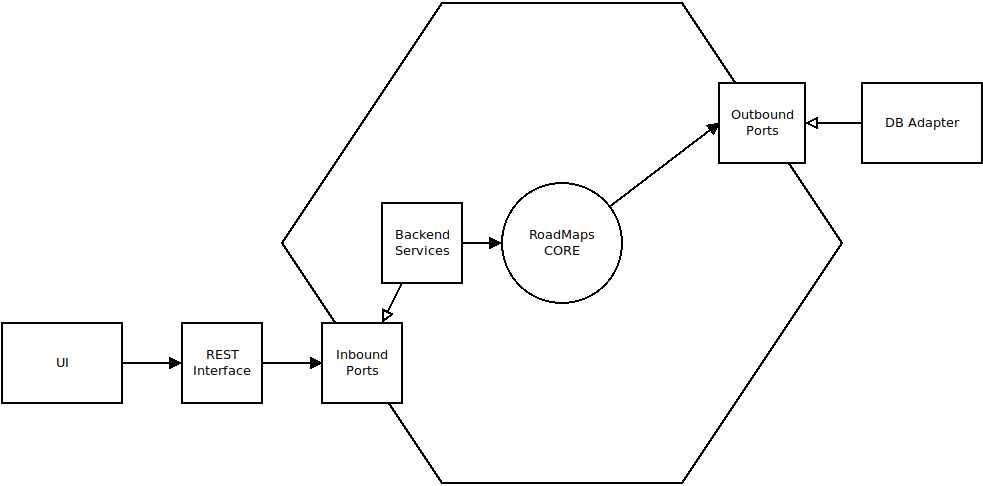
\includegraphics[width=\textwidth]{img/architecture00}
	\caption{Architettura generale}
	\label{fig:architecture00}
\end{figure}

I requisiti permettono di dividere naturalmente i servizi, le porte e gli adattatori in tre categorie:
\begin{itemize}
	\item Gestione degli utenti;
	\item Gestione delle configurazioni;
	\item Gestione dei progetti;
\end{itemize}

Un altro modulo piuttosto indipendente è quello relativo alla gestione delle analisi, ma essendo queste legate strettamente ad un progetto, saranno considerate parte dello stesso servizio.

Ognuno di questi moduli darà luogo ad un endpoint REST corrispondente ad uno o più casi d'uso, ad almeno un'entità principale e ad almeno una tabella su RDB.
Di seguito verrà riportata la descrizione di ognuno di questi blocchi partendo dal centro del modello di dominio e spostandosi all'esterno.

\subsubsection{Gestione degli utenti}
Il frammento di modello di dominio relativo alla gestione utenti è quello in figura \ref{fig:users_diagram}.

\begin{figure}[h]
	\centering
	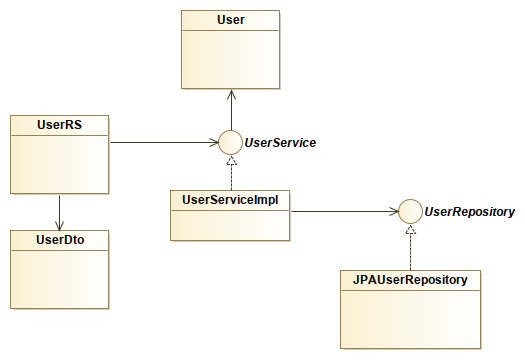
\includegraphics[width=\textwidth]{img/users_diagram}
	\caption{Diagramma delle classi relative alla gestione degli utenti}
	\label{fig:users_diagram}
\end{figure}

Dallo schema è possibile individuare quali siano le varie componenti associabili ai concetti dell'architettura esagonale:
\begin{itemize}
	\item UserService: Rappresenta una \textit{inbound port} che espone all'esterno le funzionalità relative ad un utente;
	\item UserServiceImpl: Implementa l'interfaccia \textit{UserService}, ed è quindi un \textit{inbound adapter};
	\item UserRepository: \'E una \textit{outbound port} necessaria per fornire alla logica di dominio le funzionalità di persistenza;
	\item JPAUserRepository: Implementazione di \textit{UserRepository} e quindi \textit{outbound adapter}, dipendente da una tecnologia specifica (Database relazionali + JPA), fornisce il collegamento con un RDBMS.
	\item UserRS: \'E un controller REST che espone verso il sottosistema UI i dati e le funzionalità di backend.
\end{itemize}

\subsubsection{Gestione delle configurazioni}
Il frammento di modello di dominio relativo alla gestione delle configurazioni è quello in figura \ref{fig:configurations_diagram}.

\begin{figure}[h]
	\centering
	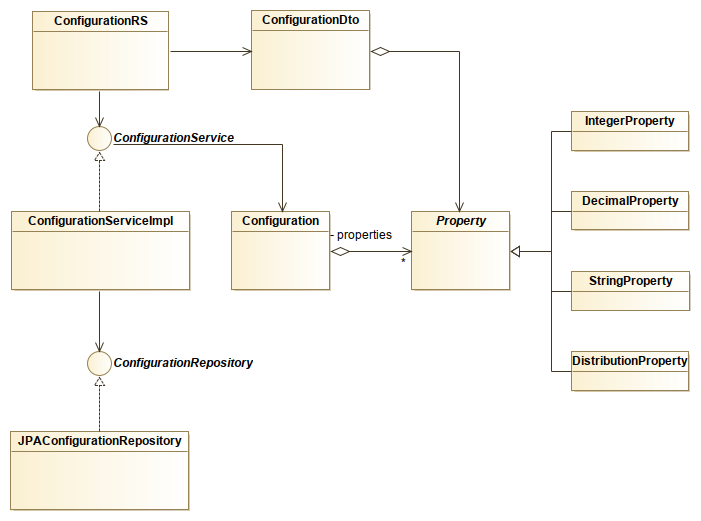
\includegraphics[width=\textwidth]{img/configurations_diagram}
	\caption{Diagramma delle classi relative alla gestione delle configurazioni}
	\label{fig:configurations_diagram}
\end{figure}

La struttura generale è equivalente a quella della sezione utenti: si hanno due interfacce \textit{ConfigurationService} e \textit{ConfigurationRepository} corrispondenti alle porte \textit{inbound} e \textit{outbound}, con i relativi adattatori \textit{ConfigurationServiceImpl} e \textit{JPAConfigurationRepository}.\\
Vi è sempre un controller REST per ricevere comandi dall'esterno del sistema, utilizzando in questo caso direttamente alcune entità del modello di dominio.

\subsubsection{Gestione dei progetti}
Il frammento di modello di dominio relativo alla gestione utenti è quello in figura \ref{fig:projects_diagram}.

\begin{figure}[h]
	\centering
	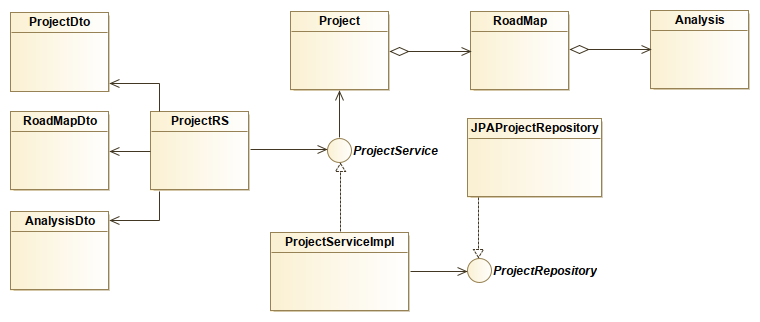
\includegraphics[width=\textwidth]{img/projects_diagram}
	\caption{Diagramma delle classi relative alla gestione dei progetti}
	\label{fig:projects_diagram}
\end{figure}

Anche in questo caso vi sono le stesse porte e adattatori più il controller REST relativo.